
    \section{基于物理模型}

    \subsection{暗通道先验}

    \begin{frame}
      \frametitle{大气散射模型}
      \begin{figure}
        \centering
        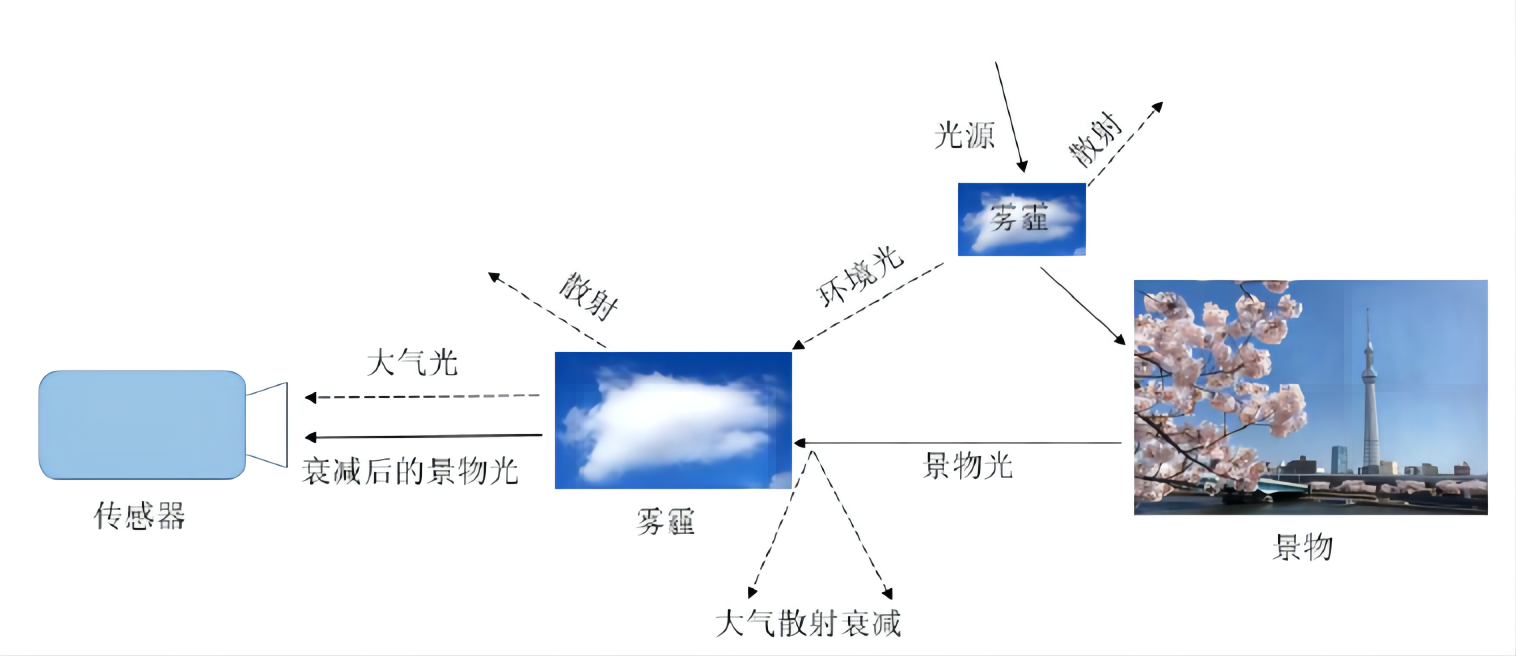
\includegraphics[width=\textwidth]{figures/pic8.png}
        \caption{大气散射模型示意图}
      \end{figure}
    \end{frame}

    \begin{frame}
      \frametitle{暗通道先验}
      对于一幅彩色图像在绝大多数非天空的局部区域里,某一些像素总会有至少一个颜色通道具有很低的值。换言之,该区域光强度的最小值是个很小的数。暗通道的数学定义为对于任意的输入图像$J$,其暗通道可以用下式表达:
      \begin{equation}
        J^{dark}(x)=\min _{y \in \Omega(x)}\left(\min _{c \in(r, g, b)} J^{c}(y)\right)
      \end{equation}
      其中,$J^c$为清晰图像$J(x)$三种色彩通道,$\Omega(x)$为图像$J(x)$中以像素$x$为中心的某一窗口,窗口大小可以根据实际情况适当调整。上式意思为:一个暗通道的值等于取一个局部窗口中每个像素点三个通道中最小值组成的集合的最小值。通过对整幅图像进行上面的操作便可以得到一幅暗通道图。
    
    \end{frame}

    \begin{frame}
      \frametitle{暗通道先验}
      作者通过大量的统计得到的先验理论指出:
      \begin{equation}
        J^{dark} \to 0
      \end{equation}
      即对于无雾的非天空部分图像的暗通道值总是趋于 0。
        
      因此,可以通过暗通道图像的最小值来估计图像的雾度。具体的,作者提出了一种基于暗通道的雾度估计方法,其数学表达式为:
      \begin{equation}
        \hat{A}=\min _{x} J^{dark}(x)
      \end{equation}
    \end{frame}

    \begin{frame}
      \frametitle{暗通道先验}
      \begin{figure}
        \centering
        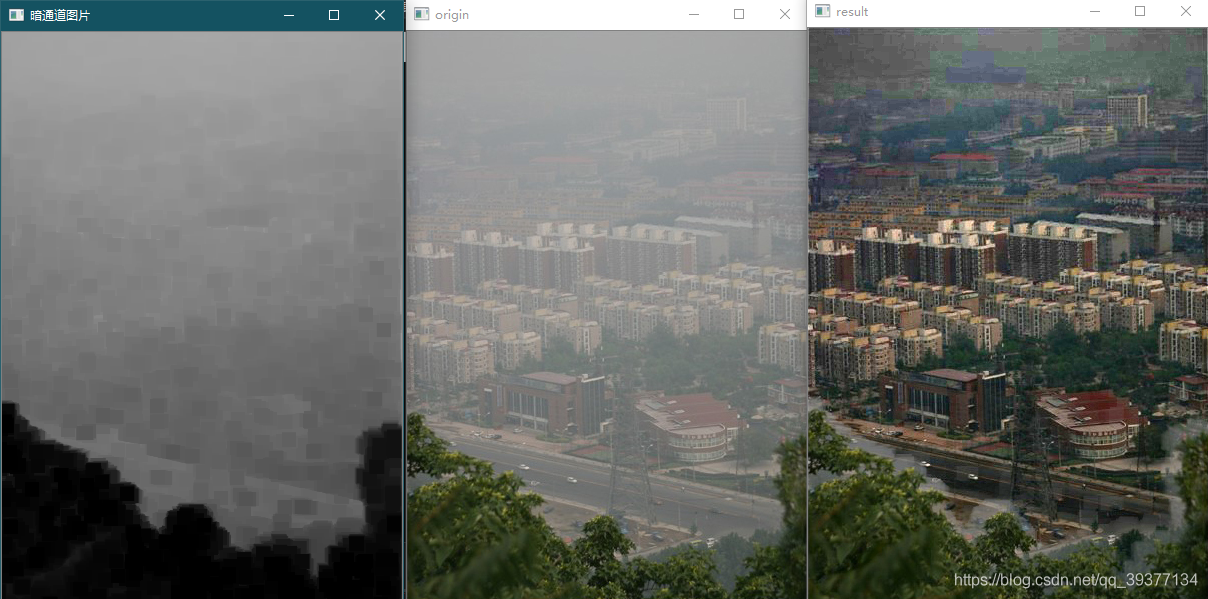
\includegraphics[width=\textwidth]{figures/pic9.png}
        \caption{暗通道先验效果图}
      \end{figure}
    \end{frame}